%!TEX root = ../bare_jrnl.tex

\section{Evaluation on Synthetic Data}
\label{sec:evasim}

We first perform an evaluation on synthetic data  to establish the benefit of POPP and its variations over the FOPP when estimating the arrival rate $\lambda$ of a Poisson process. We use synthetic data since sensor reliability can be controlled, and the true $\lambda$ and counts $c_i$ are known in advance for each observation. Our evaluation simulates two unreliable sensors across a range of conditions. In order to perform the estimation we use the switching filter from~\cite{jovan18a} across all POPP models.

In each experiment, true and false positive rates are computed based on the sampled counts $c_1, \ldots, c_n$ from a Poisson process $P(c ; \lambda'=3)$ and the corresponding sensor readings $\protect\vec{s_1} \ldots \protect\vec{s_{n}}$. 
% 
$n$ was set to 120 to limit the accuracy of the computed rates, resulting in loose Dirichlet and beta densities for the POPP-Dirichlet and the POPP-Beta models. 
% 
Another second set of counts $c_1, \ldots, c_{144}$ was sampled from the same process. These counts were then fed to simulated sensors that counted unreliably, producing sensor readings $\protect\vec{s_1} \ldots \protect\vec{s_{144}}$. A recursive update  was then performed on $P(\lambda ; \vec{s_i})$ for POPP, POPP-Beta, C-POPP, and POPP-Dirichlet models using the switching filter from~\cite{jovan18a}.

\begin{figure}[t!]
	\centering
	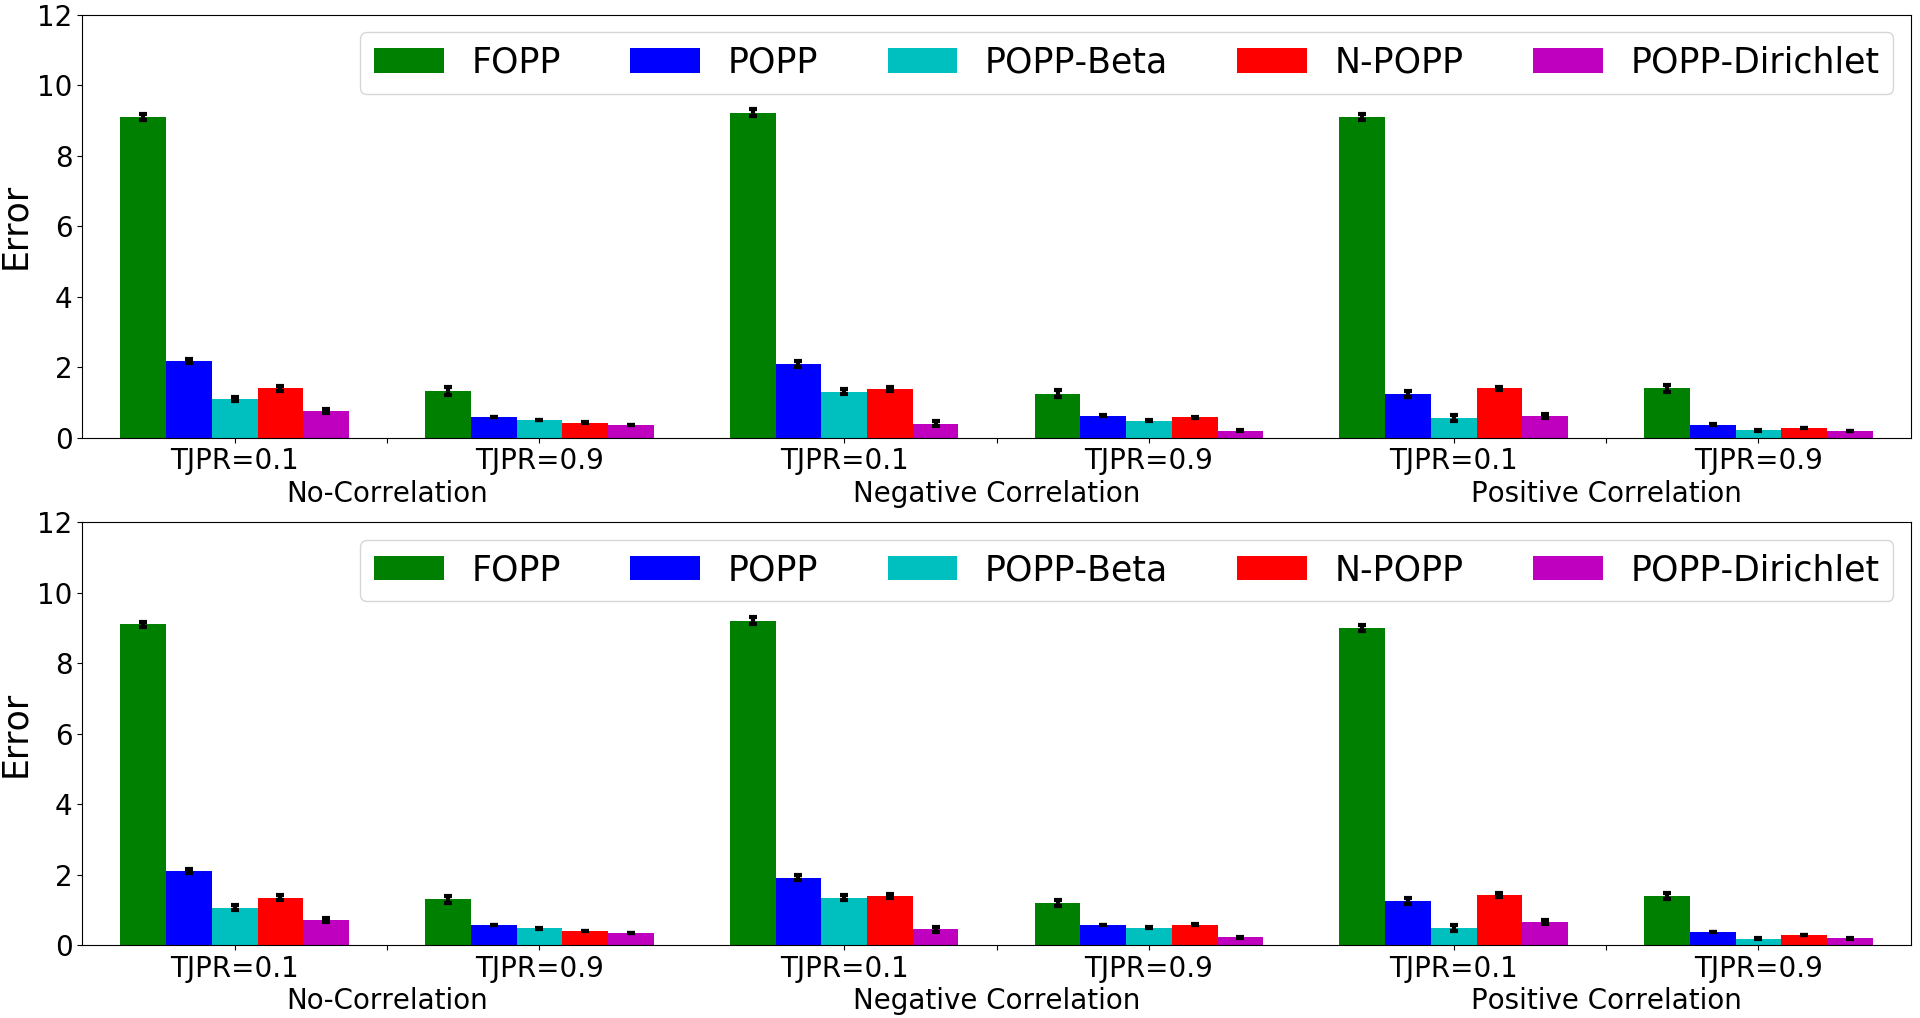
\includegraphics[width=0.5\textwidth]{./figures/tjpr_comparison_120.png}
    \caption{The RMSE of posterior estimates of $\lambda$ for the POPP and its variation models with 120 sample data used to build the (joint) sensor model with variation on $\mathcal{E^+}$. All models are compared to the FOPP model. Each trial consisted of a stream of $\protect\vec{s_1} \ldots \protect\vec{s_{144}}$ samples to update $P(\lambda ; \protect\vec{s_i})$. Accuracies of MAP estimates are shown in the top panel, accuracies of expectation of the posterior in the bottom panel. Each data point is an average of 30 trials. Standard errors are shown.} 
	\label{fig:tjpr_comparison_120}
\end{figure}

\begin{figure}[t!]
	\centering
	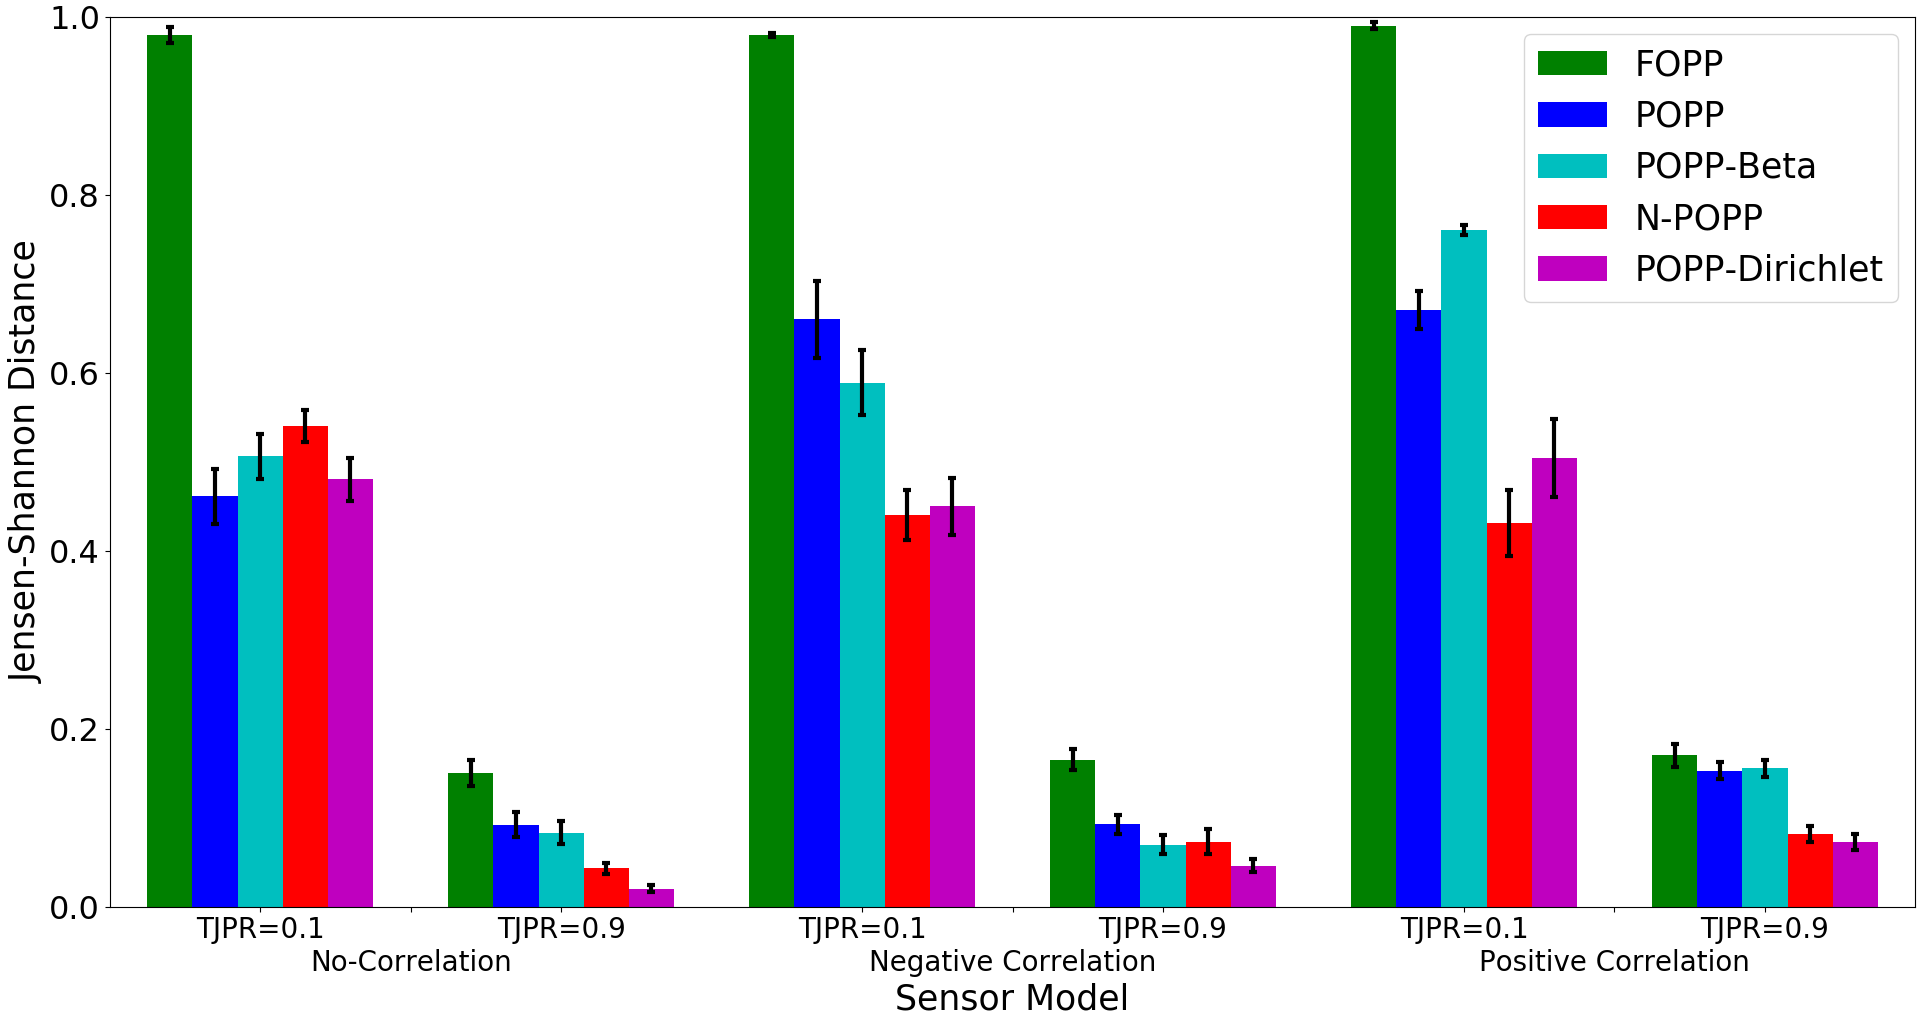
\includegraphics[width=0.5\textwidth]{./figures/tjpr_comparison_120_kl.png}
	\caption{The Jensen-Shannon distance of posterior estimates of $\lambda$ for the POPP and its variation models with 120 sample data used to build the (joint) sensor model with variation on $\mathcal{E^+}$. All models are compared to the FOPP model. Each trial consisted of a stream of $\protect\vec{s_1} \ldots \protect\vec{s_{144}}$ samples to update $P_G(\lambda \mid \protect\vec{s_i})$. Each data point is an average of 30 trials. Standard errors are shown.} 
	\label{fig:tjpr_comparison_120_kl}
\end{figure}

Different correlations between two sensors were tested: positive correlation, negative correlation, and no correlation. These correlations are designed to show the benefit of the C-POPP and POPP-Dirichlet models over the POPP and  POPP-Beta models (which assume sensors to be uncorrelated). For each correlation type, a further variation to different levels of sensor unreliability was considered. The true joint positive rate $\mathcal{E^+}$ (TJPR) and the true joint negative rate $\mathcal{E^-}$ (TJNR) were set as basis for varying sensor unreliability. For example, having TJPR configured with $P_{jnt}(d_{1k}=1, d_{2k}=1 ; e_k=1) = 0.1, P_{jnt}(d_{1k}=0, d_{2k}=0 ; e_k=1) = 0.9$ means that the true positive rate (TPR) for each sensor $j$ is $\textrm{\textit{tpr}}_j = P_j(d_k = 1; e_k=1) = 0.1$.

First, two variations were made to the true joint positive rate $\mathcal{E^+}$ (TJPR), while fixing the true joint negative rate $\mathcal{E^-}$ (TJNR) on each type of correlation. This includes:
\begin{itemize}
    \item $P_{jnt}(d_{1k}=1, d_{2k}=1 ; e_k=1) = 0.1, P_{jnt}(d_{1k}=0, d_{2k}=0 ; e_k=1) = 0.9$ ($\mathcal{E^+}$ with low positive correlation);
    \item $P_{jnt}(d_{1k}=1, d_{2k}=1 ; e_k=1) = 0.9, P_{jnt}(d_{1k}=0, d_{2k}=0 ; e_k=1) = 0.1$ ($\mathcal{E^+}$ with high positive correlation);
    \item $P_{jnt}(d_{1k}=1, d_{2k}=0 ; e_k=1) = 0.05, P_{jnt}(d_{1k}=0, d_{2k}=1 ; e_k=1) = 0.05, P_{jnt}(d_{1k}=0, d_{2k}=0 ; e_k=1) = 0.9$ ($\mathcal{E^+}$ with low negative correlation);
    \item $P_{jnt}(d_{1k}=1, d_{2k}=0 ; e_k=1) = 0.45, P_{jnt}(d_{1k}=0, d_{2k}=1 ; e_k=1) = 0.45, P_{jnt}(d_{1k}=0, d_{2k}=0 ; e_k=1) = 0.1$ ($\mathcal{E^+}$ with high negative correlation);
    \item $P_{jnt}(d_{1k}=1, d_{2k}=0 ; e_k=1) = 0.033, P_{jnt}(d_{1k}=0, d_{2k}=1 ; e_k=1) = 0.033, P_{jnt}(d_{1k}=1, d_{2k}=1 ; e_k=1) = 0.033, P_{jnt}(d_{1k}=0, d_{2k}=0 ; e_k=1) = 0.901$ ($\mathcal{E^+}$ with no correlation -- Similar to a sensor model with TPR = 0.066);
    \item $P_{jnt}(d_{1k}=1, d_{2k}=0 ; e_k=1) = 0.3, P_{jnt}(d_{1k}=0, d_{2k}=1 ; e_k=1) = 0.3, P_{jnt}(d_{1k}=1, d_{2k}=1 ; e_k=1) = 0.3, P_{jnt}(d_{1k}=0, d_{2k}=0 ; e_k=1) = 0.1$ ($\mathcal{E^+}$ with no correlation -- Similar to a sensor model with TPR = 0.6).
\end{itemize}

Second, two variations to the true joint negative rate $\mathcal{E^-}$ (TJNR), while fixing the true joint positive rate $\mathcal{E^+}$ (TJPR) on each type of correlation. This includes: 
\begin{itemize}
	\item $P_{jnt}(d_{1k}=1, d_{2k}=1 ; e_k=0) = 0.1, P_{jnt}(d_{1k}=0, d_{2k}=0 ; e_k=0) = 0.9$ ($\mathcal{E^-}$ with low positive correlation);
	\item $P_{jnt}(d_{1k}=1, d_{2k}=1 ; e_k=0) = 0.9, P_{jnt}(d_{1k}=0, d_{2k}=0 ; e_k=0) = 0.1$ ($\mathcal{E^-}$ with high positive correlation);
	\item $P_{jnt}(d_{1k}=1, d_{2k}=0 ; e_k=0) = 0.05, P_{jnt}(d_{1k}=0, d_{2k}=1 ; e_k=0) = 0.05, P_{jnt}(d_{1k}=0, d_{2k}=0 ; e_k=0) = 0.9$ ($\mathcal{E^-}$ with low negative correlation);
	\item $P_{jnt}(d_{1k}=1, d_{2k}=0 ; e_k=0) = 0.45, P_{jnt}(d_{1k}=0, d_{2k}=1 ; e_k=0) = 0.45, P_{jnt}(d_{1k}=0, d_{2k}=0 ; e_k=0) = 0.1$ ($\mathcal{E^-}$ with high negative correlation);
	\item $P_{jnt}(d_{1k}=1, d_{2k}=0 ; e_k=0) = 0.033, P_{jnt}(d_{1k}=0, d_{2k}=1 ; e_k=0) = 0.033, P_{jnt}(d_{1k}=1, d_{2k}=1 ; e_k=0) = 0.033, P_{jnt}(d_{1k}=0, d_{2k}=0 ; e_k=1) = 0.901$ ($\mathcal{E^-}$ with no correlation -- Similar to a sensor model with low TNR);
	\item $P_{jnt}(d_{1k}=1, d_{2k}=0 ; e_k=0) = 0.3, P_{jnt}(d_{1k}=0, d_{2k}=1 ; e_k=0) = 0.3, P_{jnt}(d_{1k}=1, d_{2k}=1 ; e_k=0) = 0.3, P_{jnt}(d_{1k}=0, d_{2k}=0 ; e_k=1) = 0.1$ ($\mathcal{E^-}$ with no correlation -- Similar to a sensor model with moderate TNR).
\end{itemize}

The performance of all POPP models were assessed by comparing how accurate each model is in estimating the true $\lambda'$. Two options were used to do this: (1) a distance metric method using the RMSE of the expectation (mean) and the MAP hypothesis (mode) of each model posterior distribution over $\lambda$ to the true $\lambda'$ and (2) a free-distance metric method using the Jensen-Shannon distance between the posterior distribution $P(\lambda ; \vec{s_i})$ and the distribution of the true $\lambda'$. 

\begin{figure}[t!]
	\centering
	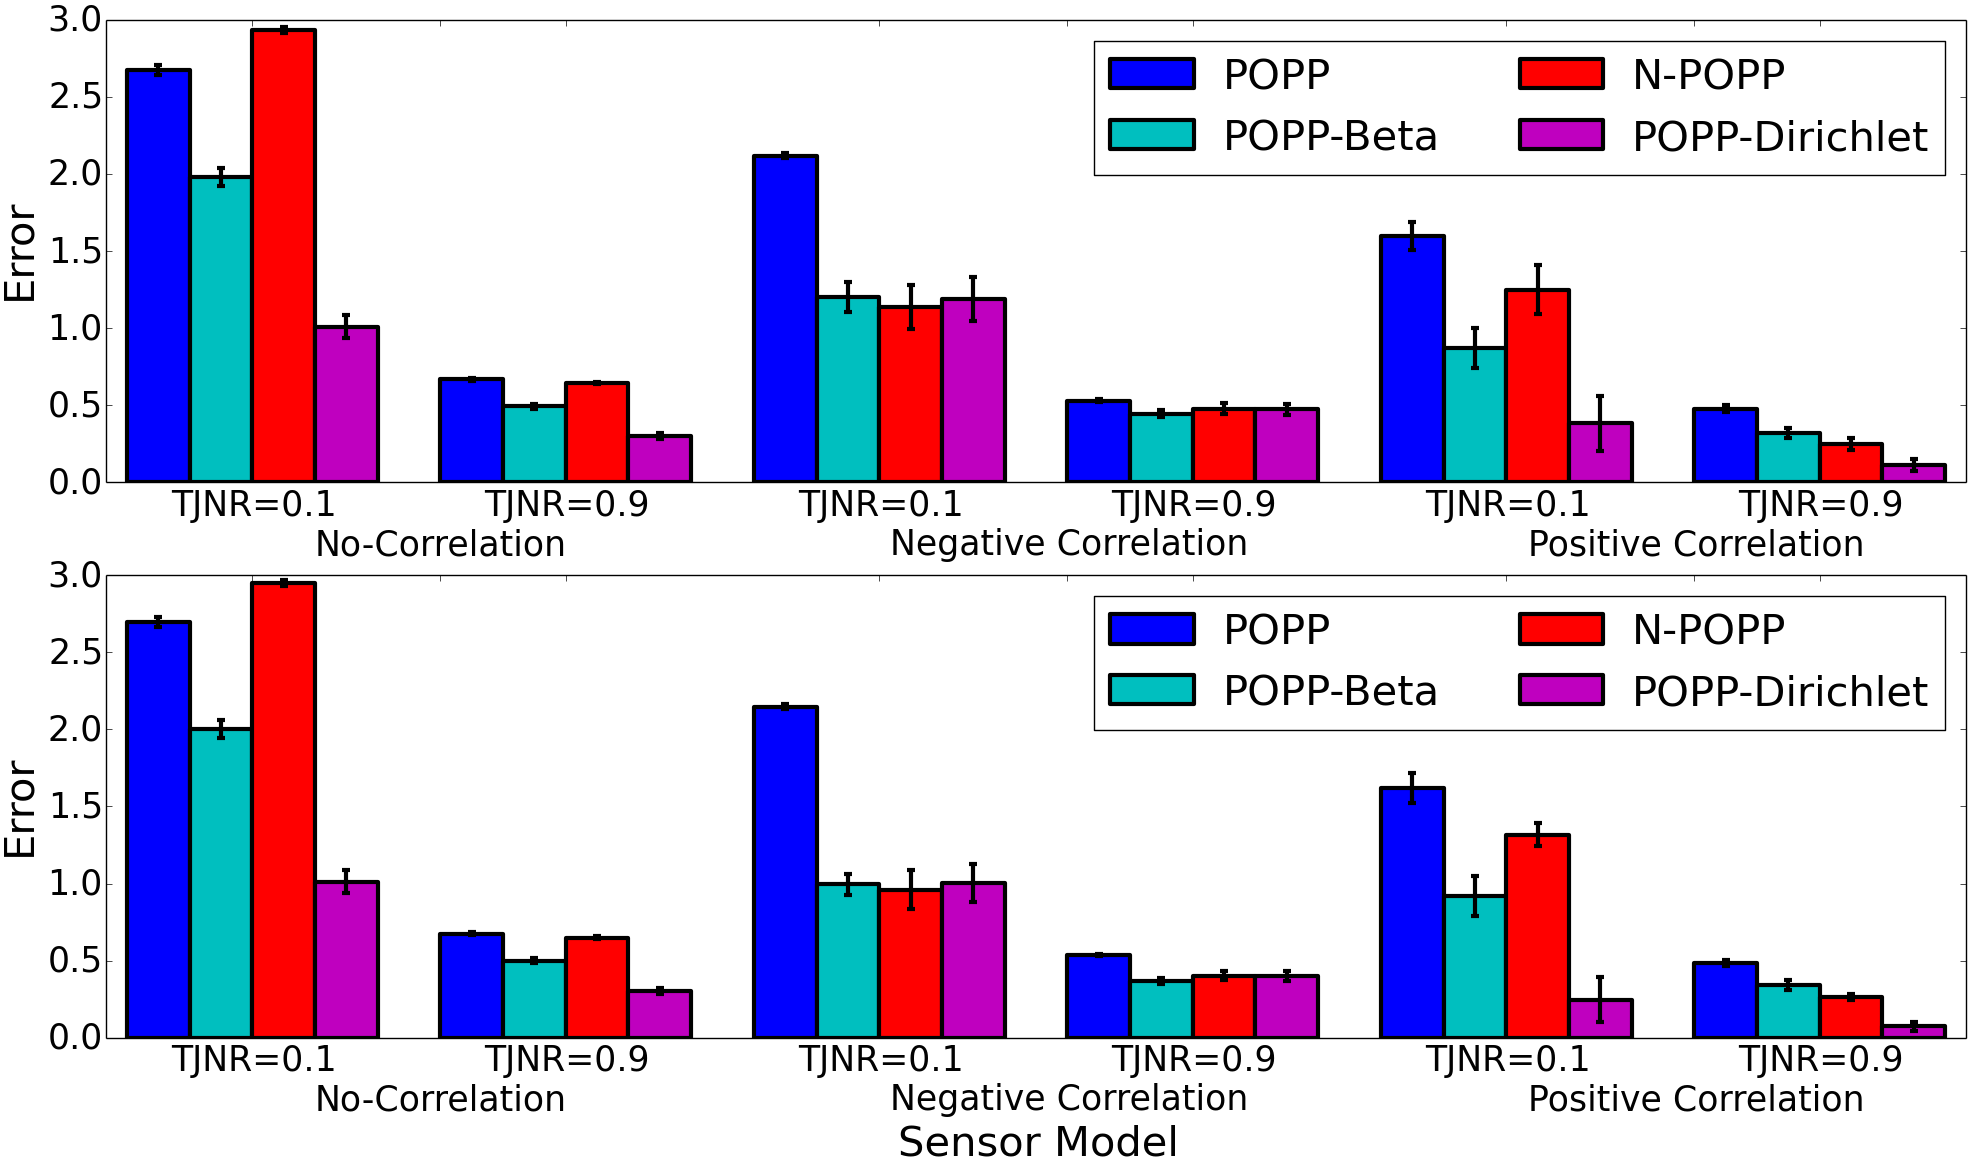
\includegraphics[width=0.5\textwidth]{./figures/tjnr_comparison_120.png}
    \caption{The RMSE of posterior estimates of $\lambda$ for the POPP and its variation models with 120 sample data used to build the (joint) sensor model with variation in $\mathcal{E^-}$. All models are compared to the FOPP model. Each trial consisted of a stream of $\protect\vec{s_1} \ldots \protect\vec{s_{144}}$ samples to update $P(\lambda ; \protect\vec{s_i})$. Accuracies of MAP estimates are  in the top panel, accuracies of the expectation of the posterior in the bottom panel. Each data point is an average of 30 trials. Standard errors are shown.} 
	\label{fig:tjnr_comparison_120}
\end{figure}

\begin{figure}[t!]
	\centering
	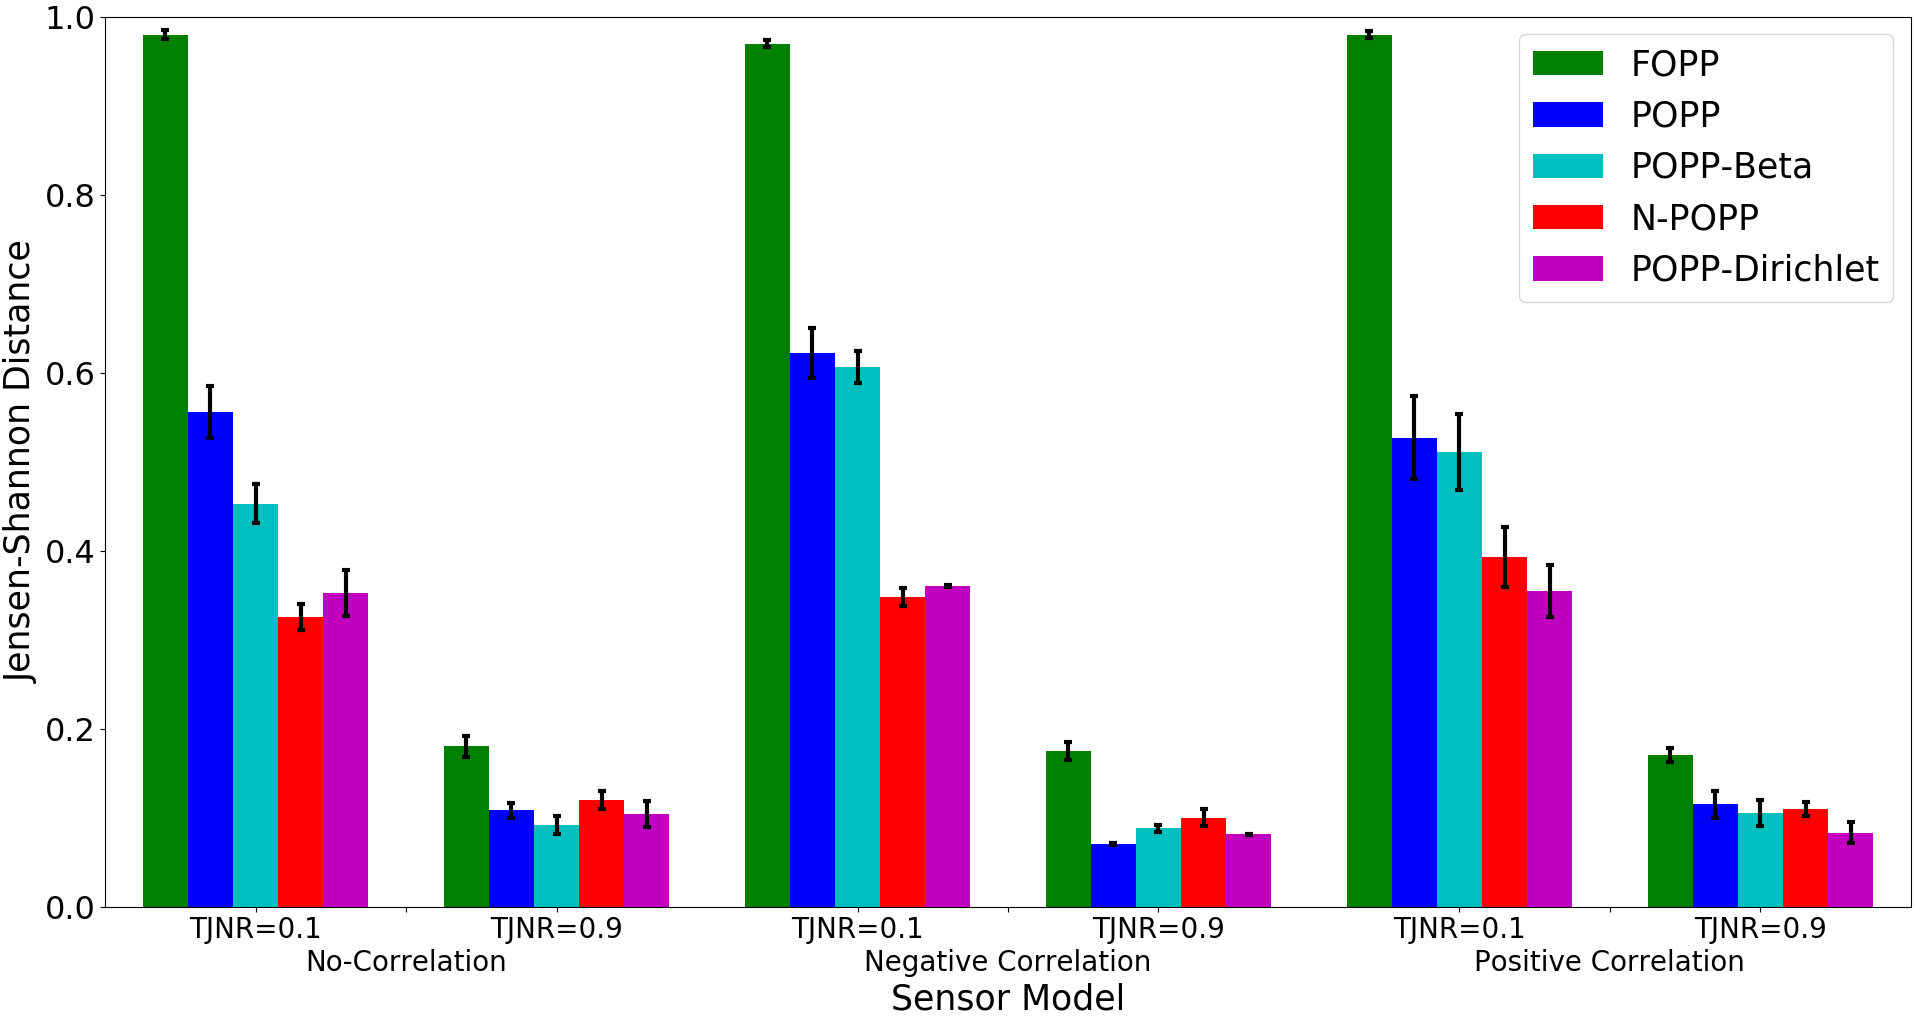
\includegraphics[width=0.5\textwidth]{./figures/tjnr_comparison_120_kl.png}
	\caption{The Jensen-Shannon distance of posterior estimates of $\lambda$ for the POPP and its variation models with 120 sample data used to build the (joint) sensor model with variation on $\mathcal{E^-}$. All models are compared to the FOPP model. Each trial consisted of a stream of $\protect\vec{s_1} \ldots \protect\vec{s_{144}}$ samples to update $P_G(\lambda \mid \protect\vec{s_i})$. Each data point is an average of 30 trials. Standard errors are shown.} 
	\label{fig:tjnr_comparison_120_kl}
\end{figure}

Figure \ref{fig:tjpr_comparison_120} and \ref{fig:tjpr_comparison_120_kl} show the accuracy of all POPP models on the variation of true joint positive rate, whereas figure \ref{fig:tjnr_comparison_120} and \ref{fig:tjnr_comparison_120_kl} show the accuracy on the variation of the true joint negative rate. From these figures, the POPP-Beta and POPP-Dirichlet show a better accuracy than the POPP and the C-POPP. The C-POPP and the POPP-Dirichlet which utilize correlation among sensors to estimate the arrival rate $\lambda'$ tend to be more accurate than the standard POPP and POPP-Beta.
In general, the POPP-Dirichlet tends to be more accurate than any other POPP model thanks to its ability to model correlation among sensors and to model how confident it is with its sensor model.
